\documentclass[10 pt,usenames,dvipsnames, oneside]{article}
\usepackage{../../../modelo-ensino-medio}



\begin{document}

\begin{center}
  \begin{minipage}[l]{3cm}

\includegraphics[width=2cm]{logo}    
\end{minipage}\hfill
\begin{minipage}[r]{.8\textwidth}
 {\Large \scshape Atividade: A Epidemia}  
\end{minipage}
\end{center}
\vspace{.2cm}

\ifdefined\prof
%Habilidades da BNCC
\begin{objetivos}
\item \textbf{EM13MAT403} Comparar e analisar as representações, em plano cartesiano, das funções exponencial e logarítmica para identificar as características fundamentais (domínio, imagem, crescimento) de cada uma, com ou sem apoio de tecnologias digitais, estabelecendo relações entre elas.
\end{objetivos}

%Caixa do Para o Professor
\begin{goals}
%Objetivos específicos
\begin{enumerate}
	\item Simular uma situação de crescimento exponencial;
	\item Reconhecer padrões exponenciais em tabelas, gráficos, identificando o papel do fator de crescimento.
\end{enumerate}

\tcblower

%Orientações e sugestões
\begin{itemize}
\item Caso deseje peça anteriormente que seus estudantes realizem uma pesquisa sobre epidemias, pandemias, endemias. Pode ser um trabalho realizado em conjunto com outras disciplinas como Geografia, Sociologia, Biologia.
	\item Esta atividade trata de um dos Temas Contemporâneos Transversais da BNCC: Saúde. E com potencial para tratar de “Vida Familiar e Social” e “Trabalho”.
	\item Para uma melhor visualização, considere organizar os estudantes em círculo
	\item É muito importante anotar os números na lousa e ir apagando à medida em que forem sendo escolhidos, para ajudar os novos infectados a escolher suas vítimas.
	\item Escolha um estudante para ser o pesquisador e anotar os dados no quadro.
	\item Ao final de cada rodada pergunte à turma como evoluiria o total de infectados nas próximas rodadas caso houvesse mais alunos na turma.
	\item Para responder o item (e) você pode consultar a população da sua cidade e estado neste link (\url{https://www.ibge.gov.br/estatisticas/sociais/populacao/9103-estimativas-de-populacao.html?=&t=resultados})
	\item Adaptado de BUSH, S., GIBBONS, K., KARP, K., DILLON, F. Epidemics, exponential function and modelling, Mathematics Teaching in the Middle School, Vol. 21, No. 2, pp. 90-97, 2015.
\end{itemize}
\end{goals}

\bigskip
\begin{center}
{\large \scshape Atividade}
\end{center}
\fi

Vamos simular três situações de epidemia. O professor irá distribuir envelopes contendo um número para cada estudante que deverá mantê-lo em segredo. Os primeiros infectados serão escolhidos ao acaso pelo professor. Cada vez que alguém for infectado pela doença, coloca-se de pé e permanece até o fim da dinâmica, que seguirá da seguinte maneira:

\begin{figure}[H]
\centering
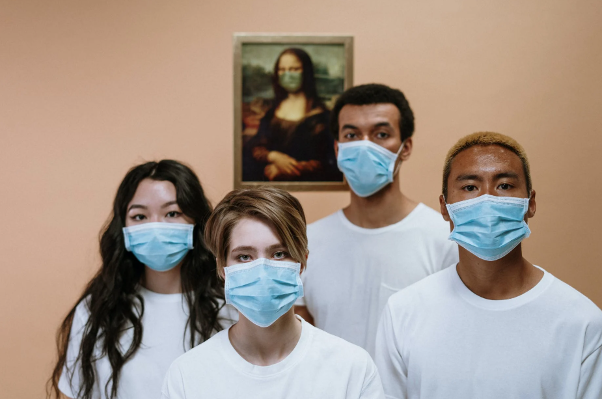
\includegraphics[width=275bp]{epidemia.png}
%\caption{https://youtu.be/s-lgS-4Xqy0}
\end{figure}


\paragraph{Epidemia 1}

\begin{itemize}

\item RODADA 0: O professor escolhe dois números para serem os primeiros infectados, diz seus números e apaga-os da lista que está escrita na lousa. Os infectados ficam de pé. O pesquisador anota o número de infectados.

\item RODADA 1: Cada um dos infectados escolhe um número que não tenha sido sorteado para “infectar”; os números são apagados na lousa e somente depois de todos terem escolhido suas vítimas, os novos infectados se colocam de pé. O pesquisador anota o número total de infectados.

\item RODADA 2: Semelhante à rodada 1.

\item As rodadas seguem até que todos tenham sido infectados.

\end{itemize}

% 

\paragraph{Epidemia 2}

\begin{itemize}

\item A mesma dinâmica anterior, porém começando com três infectados na rodada 0.

\end{itemize}

\paragraph{Epidemia 3}
\begin{itemize}

\item Apenas um infectado na rodada 0 e cada infectado agora escolhe dois números para infectar a cada rodada.

\end{itemize}

Responda às seguintes perguntas:

\begin{enumerate}
\item{} 
Anote os dados das três epidemias em tabelas e faça previsões para 4 rodadas além das que efetivamente ocorreram na sua turma.

\item{} 
Represente os dados graficamente.

\item{} 
Que critérios você usou no item (a) para fazer suas previsões? Qual a relação deles com os dados específicos de cada uma das epidemias.

\item{}
Quantas rodadas aproximadamente demoraria para cada epidemia infectar todos os estudantes da sua escola? Primeiro faça um “chute” e somente depois faça as contas.

\item{}
Responda a mesma pergunta anterior considerando a sua cidade, seu estado e o todo o país.

\end{enumerate}

\ifdefined\prof
\begin{solucao}

\begin{enumerate}
\item {} 
Tabela com o número de infectados até a rodada 8.

\begin{tabular}{|c|c|c|c|}
\hline
\tcolor{Rodada} & \tcolor{Epidemia 1} & \tcolor{Epidemia 2} & \tcolor{Epidemia 3} \\ \hline
0      & 2          & 3          & 1          \\ \hline
1      & 4          & 6          & 3          \\ \hline
2      & 8          & 12         & 9          \\ \hline
3      & 16         & 24         & 27         \\ \hline
4      & 32         & 48         & 81         \\ \hline
5      & 64         & 96         & 243        \\ \hline
6      & 128        & 192        & 729        \\ \hline
7      & 256        & 384        & 2187       \\ \hline
8      & 512        & 768        & 6561       \\ \hline
\end{tabular}

\item\adjustbox{valign=t}
{
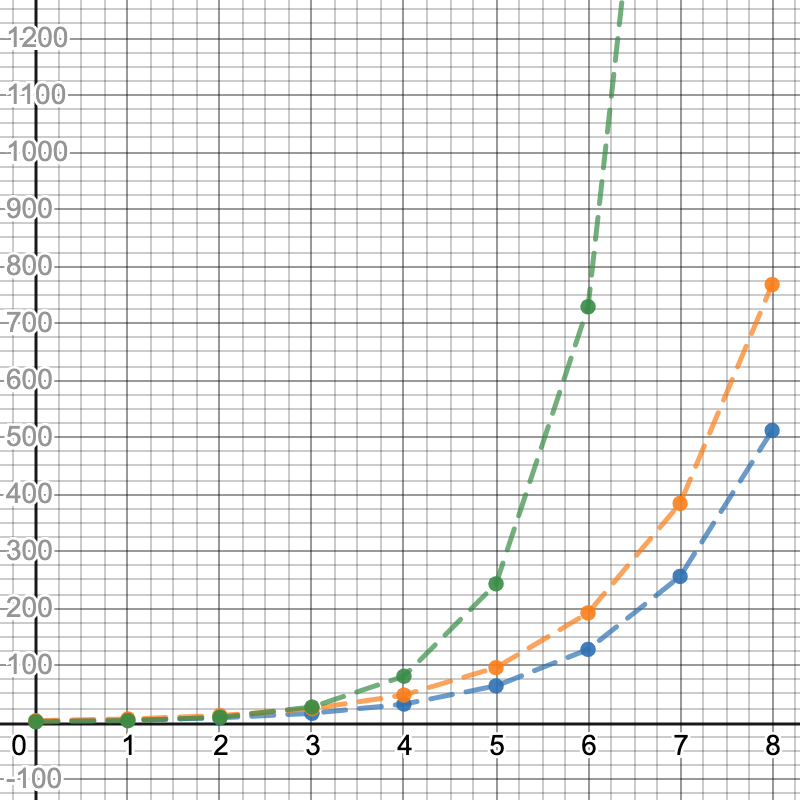
\includegraphics[width=.7\linewidth]{epidemias.png}
}

\item{}
Uma resposta possível é dizer que nas epidemias $1$ e $2$ a cada rodada o número de infectados dobra. Na epidemia $3$ o número de infectados triplica a cada rodada.

\item{}
A informação solicitada depende do número de estudantes da escola.

\item{}
As informações solicitadas dependem de informações sobre a população da cidade, estado e país.
\end{enumerate}

\end{solucao}
\fi

\end{document}